% The weekly review's two layers: scripts on a clock, and an assistant that can
% only enter the bibliography through a verifier.
% ---------------------------------------------------------------------------
% style.tex --- shared preamble for every figure in book/figures/tikz/
%
% One style for all figures: Latin Modern, thin black lines, a light grey
% fill, and one accent colour used only to mark what is untrusted or wrong.
% Build with scripts/build_figures.sh; see book/figures/README.md.
% ---------------------------------------------------------------------------
\documentclass[tikz,border=6pt]{standalone}
\usepackage[T1]{fontenc}
\usepackage{lmodern}
\usetikzlibrary{arrows.meta,positioning,shapes.geometric,calc,fit,backgrounds}

\hyphenpenalty=10000   % short lines in boxes: ragged, never hyphenated

\definecolor{lightgrey}{gray}{0.92}
\definecolor{accent}{HTML}{9B2D20}

\tikzset{
  every picture/.style={
    line width=0.6pt,
    font=\small,
    >={Stealth[length=5pt,width=4pt]},
    node distance=14pt and 24pt,
  },
  % shapes
  box/.style={draw, rectangle, inner xsep=8pt, inner ysep=5pt,
              minimum height=22pt, align=center},
  grey/.style={box, fill=lightgrey},
  rounded/.style={box, rounded corners=9pt},
  decision/.style={draw, diamond, aspect=2.4, inner sep=1.5pt, align=center},
  group/.style={draw, dashed, rounded corners=5pt, inner sep=7pt},
  % text
  tag/.style={font=\footnotesize, align=center, inner sep=2pt},
  note/.style={font=\footnotesize\itshape, align=center, inner sep=2pt},
  code/.style={font=\small\ttfamily},
  codetag/.style={font=\footnotesize\ttfamily, align=center, inner sep=2pt},
  title/.style={font=\small\scshape, align=center, inner sep=2pt},
  % lines
  arrow/.style={->},
  back/.style={->, dashed},
  thin/.style={line width=0.4pt, gray},
  % the one accent, for what is untrusted, wrong or missing
  bad/.style={accent},
  badbox/.style={box, draw=accent, text=accent},
}

\begin{document}
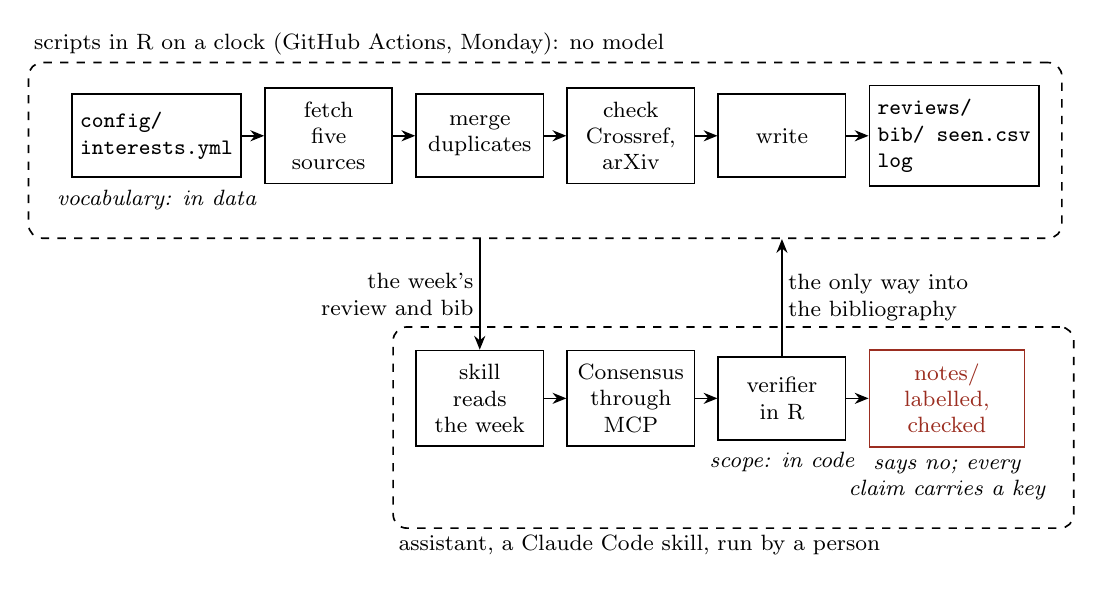
\begin{tikzpicture}[node distance=10pt and 8pt,
                    st/.style={box, text width=40pt, inner xsep=3pt, align=center, font=\footnotesize, minimum height=30pt},
                    f/.style={box, font=\footnotesize\ttfamily, inner xsep=3pt, align=left, minimum height=30pt}]
  % scripts
  \node[f] (cfg) {config/\\interests.yml};
  \node[st, right=of cfg] (fetch) {fetch\\five sources};
  \node[st, right=of fetch] (norm) {merge\\duplicates};
  \node[st, right=of norm] (check) {check\\Crossref, arXiv};
  \node[st, right=of check] (write) {write};
  \node[f, right=of write] (out) {reviews/\\bib/ seen.csv\\log};
  \draw[->] (cfg) -- (fetch); \draw[->] (fetch) -- (norm); \draw[->] (norm) -- (check); \draw[->] (check) -- (write); \draw[->] (write) -- (out);
  \node[note, below=2pt of cfg] (n1) {vocabulary: in data};
  \node[group, fit=(cfg) (out) (n1), inner xsep=8pt, inner ysep=8pt] (top) {};
  \node[tag, anchor=south west] at (top.north west) {scripts in R on a clock (GitHub Actions, Monday): no model};
  % assistant
  \node[st, below=62pt of norm] (skill) {skill\\reads the week};
  \node[st, right=of skill] (cons) {Consensus\\through MCP};
  \node[st, right=of cons] (ver) {verifier\\in R};
  \node[badbox, right=of ver, text width=50pt, inner xsep=3pt, align=center, font=\footnotesize, minimum height=30pt] (notes) {notes/\\labelled, checked};
  \draw[->] (skill) -- (cons); \draw[->] (cons) -- (ver); \draw[->] (ver) -- (notes);
  \draw[->] (skill.north |- top.south) -- node[tag, left, align=right] {the week's\\review and bib} (skill.north);
  \draw[->] (ver.north) -- node[tag, right, align=left] {the only way into\\the bibliography} (ver.north |- top.south);
  \node[note, below=2pt of ver] (n2) {scope: in code};
  \node[note, below=2pt of notes] (n3) {says no; every\\claim carries a key};
  \node[group, fit=(skill) (notes) (n2) (n3), inner xsep=8pt, inner ysep=8pt] (bot) {};
  \node[tag, anchor=north west] at (bot.south west) {assistant, a Claude Code skill, run by a person};
\end{tikzpicture}
\end{document}
